% ===== 09_population =====
\section{参照指标与有效人口比较}
\label{sec:sup:population}
\subsection{设定与比较基准}
\label{sec:dom:setup}

本节比较仅隔离控制与固定 TDINN 参照。数值情景固定绝对初值，理论尺度关系固定归一化初值。记
\begin{equation}
  \theta:=\frac{\eta}{N}\quad(\text{阈值比例}),\qquad
  i_{\max}^{no}:=\frac{I_{\max}^{no}}{N}\quad(\text{常规控制峰值比例}),
  \label{eq:dom:ratios}
\end{equation}
其中 $I_{\max}^{no}$ 由式~\eqref{eq:s1:Imax-no} 给出。在归一化初值 $s_0=S_0/N$ 与 $i_0=I_0/N$ 固定时，
$S_c,\bar S,I_{\max}^{no}$ 均随 $N$ 同比例缩放，故 $i_{\max}^{no}$ 不依赖 $N$，
只依赖 $\beta,\gamma,c_0,q_0,s_0,i_0$。本节记归一化状态 $s=S/N$、$i=I/N$。

数值情景取 $N=N_{\rm eff}$、$S_0=N-I_0$，其余初始仓室为零，$I_0$ 固定为全市拟合的未取整值，不重新拟合。人口必要下界 $N_{\rm floor}$ 见正文命题\ref{prop:dom:floor}。由首次积分，$i_0$ 通过 $\theta-i_0$ 和 $s_0=1-i_0$ 影响启动点。在 $N\ge N_{\rm floor}$、$\theta\ge\theta_{\rm dur150}$ 时，$i_0/\theta$ 不超过约 $8.3\times10^{-5}$；该比例本身不是控制指标的严格误差上界。

TDINN 的四个参照量固定为全市人口下的重构结果（表\ref{tab:xian_summary}），其二次成本采用 $w_c=1,w_q=2$。仅隔离控制的累计新增感染统计至自身的清零终点，$J$ 只计阈值控制期的二次成本。$\Delta t$ 为控制时长，$t_{\rm end}$ 为从共同时间原点起算的清零时间。


\subsection{仅隔离控制的比较条件}
\label{sec:dom:theory}
命题\ref{prop:scaling}已给出固定归一化初值时的规模不变性。以下理论条件及式\eqref{eq:dom:Nstar}、\eqref{eq:dom:Nstar-infty}的商式仍以这一初值约定为前提；固定绝对 $I_0$ 的应用上界在第\ref{sec:dom:xian}节按实际指标求根定义，不直接由这些商式确定。

由命题\ref{prop:threshold-tradeoff}，$\Delta t(\theta)$、$J(\theta)$ 随 $\theta$ 严格递减。给定 $J^{\rm T}>0$ 和 $T_{\max}>0$，在相应值域内定义
\begin{equation}
J(\theta_{\rm cost})=J^{\rm T},\qquad
\Delta t\bigl(\theta_{\rm dur}(T_{\max})\bigr)=T_{\max},
\label{eq:dom:thetadefs}
\end{equation}
并记
\begin{equation}
\theta_{\rm bind}(T_{\max})
=\max\{\theta_{\rm cost},\theta_{\rm dur}(T_{\max})\}.
\label{eq:dom:theta-bind}
\end{equation}
当某项限制对全部内部触发阈值都成立时，相应阈值延拓为 $i_0$；完整定义见第\ref{app:reference-comparison}节。于是同时满足峰值 $\eta\le I^{\rm T}_{\rm peak}$、成本 $J\le J^{\rm T}$ 和时长 $\Delta t\le T_{\max}$ 的阈值比例集合为
\begin{equation}
(i_0,i_{\max}^{no})\cap
\left[\theta_{\rm bind}(T_{\max}),\frac{I^{\rm T}_{\rm peak}}N\right].
\label{eq:dom:band}
\end{equation}
在 $\theta_{\rm bind}>i_0$ 且 $\theta_{\rm bind}<i_{\max}^{no}$ 时，该集合非空等价于
\begin{equation}
N\le N^*(T_{\max}):=\frac{I^{\rm T}_{\rm peak}}{\theta_{\rm bind}(T_{\max})}.
\label{eq:dom:Nstar}
\end{equation}
若 $\theta_{\rm bind}=i_0$，则需改为 $N<I^{\rm T}_{\rm peak}/i_0$，以排除初始时刻直接处于阈值的端点。固定正 $i_0$ 时，增大 $T_{\max}$ 只会使时长条件最终不再起限制作用；$\theta_{\rm dur}$ 的端点极限是 $i_0$，不能写成零。成本阈值位于内部时，不再限制时长所对应的界值仍为
\begin{equation}
N^*_{\infty}=\frac{I^{\rm T}_{\rm peak}}{\theta_{\rm cost}}.
\label{eq:dom:Nstar-infty}
\end{equation}
式\eqref{eq:dom:band}同时施加峰值、二次成本和控制时长条件，累计新增感染及清零时间需按下节的实际指标另行比较。

\subsection{附加指标与规模关系}
\label{sec:dom:extra}
进一步加入累计新增感染和社区清零时间条件时，分别计算
\begin{equation}
\Itcum(\eta,N)=\Itcum^{\rm T},
\label{eq:dom:cumarc}
\end{equation}
\begin{equation}
t_{\rm end}(\eta,N)=t_{\rm end}^{\rm T}.
\label{eq:dom:clrarc}
\end{equation}
两项指标均采用绝对清零终点 $I=1$，其等值条件因而不只依赖 $\eta/N$。它们与式\eqref{eq:dom:band}及人口下界共同限定比较范围。固定归一化初值和固定 $\theta$ 时，人口单调性由命题\ref{prop:reference-population}给出；固定绝对初值、固定 $\eta$ 的等值线则按实际指标计算。

沿用原记号，以 $N^*_{\rm cum}(T_{\max})$ 表示相应参数计算中累计新增感染等值线与起约束作用的阈值条件的交点，以 $N_{\rm clr}(\eta)$ 表示清零等值线在固定 $\eta$ 时对应的人口。若交点有多个，则须保留全部交点并逐段判断；以下单条边界及界值均指当前数值范围中的结果。记 $N^*_{\rm cum,\infty}$ 为不另设控制时长上限的对应值。第\ref{app:dom:numerics}节保留计算点和适用范围说明。


\subsection{规模关系的数值说明}
\label{sec:scaling}
固定绝对初值的既有参数点显示，固定阈值比例时控制时长近似不变，固定绝对阈值时随人口增加。命题\ref{prop:scaling}固定归一化初值，以下只比较数值尺度关系。

固定 $\theta=0.002$，取 $N_{\rm eff}\in\{5\times10^4,\dots,1.316\times10^7\}$。六个人口规模下的控制时长均约为 $85.07$ 天，$\Delta t$ 和 $J$ 的相对极差分别为 $4.71\times10^{-8}$ 和 $1.17\times10^{-7}$。以 $t-t_1$ 为时间变量时，归一化感染轨迹和隔离比例近似重合；这些结果不提供所有初值或人口下的统一误差界。启动时间由 $11.39$ 天增加至 $16.90$ 天，这是固定绝对初值、初始感染比例随 $N$ 变化的结果。

固定绝对阈值 $\eta=100$，把 $N_{\rm eff}$ 从 $1.316\times10^7$ 降到 $5\times10^4$，则 $\theta=\eta/N_{\rm eff}$ 增大，控制时长由约 $2.25\times10^4$ 天缩短到约 $85$ 天。两组结果中，控制时长主要随 $\theta$ 变化：
\[
\Delta t=\frac1{c_0\theta}\ln\frac{s^*-\bar s}{s_c-\bar s}.
\]
对数因子在 $\theta\in[5\times10^{-4},8\times10^{-3}]$ 内仅由 $2.20$ 变到 $2.15$，因此在该范围内 $\Delta t$ 近似与 $\theta$ 成反比。

固定 $\beta=0.1498$，在 $\eta\in\{80,100,150\}$、$N_{\rm eff}\in\{4,5,6\}\times10^4$ 的九组参数中，将解析拐点时刻回代开环控制，所得隔离比例均约为 $0.4119$。该结果为解析公式回代，不是独立 ODE 积分验证。当 $q_0=0.3230$ 时，$\qinf=q_0$ 给出 $\beta_{\max}=0.261448$；超过该值后控制区间内不再有内部拐点。

\subsection{西安参数下的比较条件与候选范围}
\label{sec:dom:xian}

峰值、成本和时长条件给出不同的数值求根值，加入累计新增感染或清零时间后，比较范围还会缩小。沿用正文表\ref{tab:xian_initial_fit}的传播参数和本节的固定绝对初值，取全市参考人口 $N_{\rm ref}=13{,}163{,}000$。由式\eqref{eq:s1:Imax-no}得该人口下 $i_{\max}^{no}\approx0.1047$；所考察的 $T_{\max}=45,60,90,150$ 天及不限制时长的设定均有 $\theta_{\rm bind}<i_{\max}^{no}$。

表\ref{tab:dom:thresholds}中的界值分别对应人口必要条件、数值求根和有限扫描结果。在全市参考人口下，$T_{\max}\approx103$ 天时有 $\theta_{\rm dur}=\theta_{\rm cost}$。更短的允许时长使时长条件起约束作用，更长的允许时长则由成本条件决定阈值下限。


\begin{table}[htbp]
\centering\small
\setlength{\tabcolsep}{3.5pt}
\renewcommand{\arraystretch}{1.25}
\begin{threeparttable}
\caption{不同指标限制对应的有效人口界值}
\label{tab:dom:thresholds}
\begin{tabularx}{\linewidth}{@{}>{\raggedright\arraybackslash}p{0.27\linewidth}>{\centering\arraybackslash}p{0.21\linewidth}>{\centering\arraybackslash}p{0.16\linewidth}>{\raggedright\arraybackslash}X@{}}
\toprule
比较条件 & 相关量 & 数值（人） & 与人口下界的关系\\
\midrule
人口相容条件 & $N_{\rm floor}$ & $1.06\times10^4$ & 比较时施加的下界\\
峰值、成本及45 d时长条件 & $N^*(45\,\mathrm d)$ & $4.06\times10^4$ & 对应上界高于下界\\
峰值与成本，不另设时长上限 & $N^*_{\infty}$ & $9.22\times10^4$ & 对应上界高于下界\\
再加入累计新增感染条件 & $N^*_{\rm cum,\infty}$ & $1.18\times10^4$ & 数值界值接近下界\\
清零时间等值条件 & \makecell{$N_{\rm clr}(\eta)$\\的最大取值} & 5184 & 扫描范围内仍低于下界\\
\bottomrule
\end{tabularx}
\begin{tablenotes}[flushleft]\footnotesize
\item 注：前四项为近似值。后两行对应本文西安参数、固定绝对初值和 $\eta\in[10,152.55]$ 的数值范围，不表示已证明任意参数下的交点唯一性或全局人口上界。
\end{tablenotes}
\end{threeparttable}
\end{table}

固定绝对初值时，峰值、成本、时长和触发条件在 $(N,\eta)$ 平面上的边界分别为
\begin{align}
  \text{峰值线：}\ &
  \eta=I_{\rm peak}^{\rm T}
  &&(\text{占优侧 }\eta\le I_{\rm peak}^{\rm T}),\\
  \text{成本边界：}\ &
  J(\eta,N)=J^{\rm T}
  &&(\text{占优侧 }J(\eta,N)\le J^{\rm T}),\\
  \text{时长边界：}\ &
  \Delta t(\eta,N)=T_{\max}
  &&(\text{占优侧 }\Delta t(\eta,N)\le T_{\max}),\\
  \text{触发边界：}\ &
  \eta=I_{\max}^{no}(N)
  &&(\text{可行侧 }\eta<I_{\max}^{no}(N)).
\end{align}
其中 $J(\eta,N)$、$\Delta t(\eta,N)$ 和 $I_{\max}^{no}(N)$ 均按同一个绝对初值 $I_0$ 与 $S_0=N-I_0$ 计算，其余模型参数不变；$S_0$ 与 $S_c=\gamma N/[\beta c_0(1-q_0)]$ 均随 $N$ 改变。比较集合按实际指标定义为
\[
\mathcal{W}_{\rm pcd}
=
\left\{
(N,\eta):
\begin{array}{l}
N>I_0,\quad S_0>S_c,\quad I_0<\eta<I_{\max}^{no}(N),\\
\eta\le I_{\rm peak}^{\rm T},\\
J(\eta,N)\le J^{\rm T},\quad\Delta t(\eta,N)\le T_{\max}
\end{array}
\right\}.
\]
不另设时长上限时去掉最后的时长条件；人口相容下界仍在后文与该集合取交。峰值线是精确的水平线。图~\ref{fig:dom}中的成本、时长和触发参考直线采用全市参考人口 $N_{\rm ref}$ 下的未取整比例；固定绝对初值时，这些比例随 $N$ 改变，图中直线只显示比较区域的近似形状。集合归属和临界点均以实际成本、时长及严格触发条件判断，不以参考直线代替。

比较区域的阈值下限由实际成本与时长条件共同确定。仅当两项允许人口集合分别为截止于相应界值的连续区间时，共同上界 $N^\ast(T_{\max})$ 才取两者上界的较小者，不要求二者同时取等号。现有结果保存了数值求根值和代表轨迹，尚未确认整个人口允许集合的区间结构；表~\ref{tab:dom:thresholds}中的人口界值据此作为候选上界，不作一般唯一性或单一区间的断言。这一应用判断不同于第\ref{sec:dom:theory}节固定归一化初值下的商式。所报告的数值交点满足 $I_0<I_{\rm peak}^{\rm T}<I_{\max}^{no}(N)$；例如，$152.55$ 远小于 $I_{\max}^{no}(N^\ast_\infty)\approx9.6\times10^{3}$，严格触发条件未被取等号。

图~\ref{fig:dom}(a) 近似展示上述比较区域的形状，图~\ref{fig:dom}(b) 加入累计新增感染和清零时间条件，对应集合为
\[
\mathcal{W}_{\rm cum}=\mathcal{W}_{\rm pcd}\cap\{\Itcum\le \Itcum^{\rm T}\}\cap\{N\ge N_{\rm floor}\},
\qquad
\mathcal{W}_{\rm clr}=\mathcal{W}_{\rm pcd}\cap\{t_{\rm end}\le t_{\rm end}^{\rm T}\}
\cap\{N\ge N_{\rm floor}\},
\]
其中施加同一人口相容下界 $N\ge N_{\rm floor}$。在本文参数及扫描范围内，
$\mathcal{W}_{\rm clr}\subset\mathcal{W}_{\rm cum}\subset\mathcal{W}_{\rm pcd}$。


\begin{figure}[htbp]
\centering
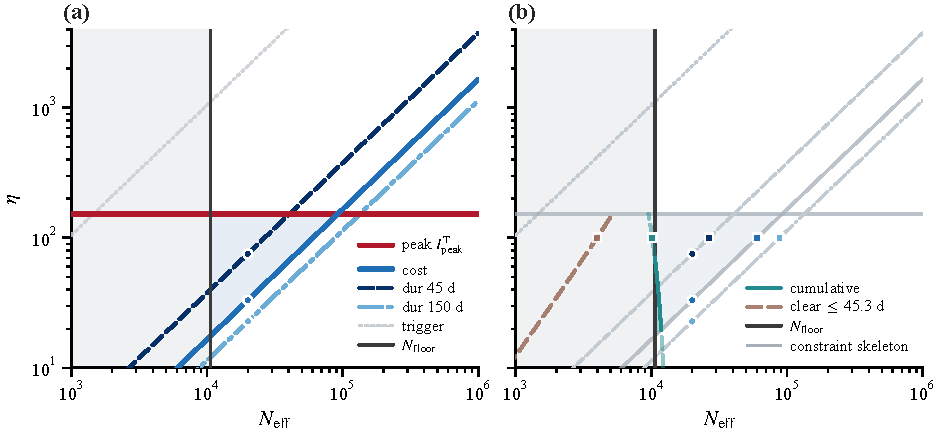
\includegraphics[width=\textwidth]{figures/fig_dom_combined.pdf}
\caption{西安参数下 $(N_{\rm eff},\eta)$ 平面比较区域的近似展示。(a) 峰值条件及成本、时长和触发参考直线；后三者采用 $N_{\rm ref}=13{,}163{,}000$ 下的未取整比例。人口下界右侧的浅蓝区域示意峰值、成本与触发条件的交集，未另加时长上限；左侧灰色区域因 $N<N_{\rm floor}$ 被排除。(b) 加入累计新增感染和清零时间的等值曲线。竖直实线为 $N_{\rm floor}=1.06\times10^4$。计算所得累计新增感染与成本条件的交点约为 $(11813,19.55)$，清零时间等值曲线位于人口下界左侧。圆点和方点分别示意固定人口改变阈值、固定阈值改变人口的两类比较；轨迹案例的具体参数见图\ref{fig:dom:levers}(a,c)、\ref{fig:dom:levers}(b,d)。}
\label{fig:dom}
\end{figure}


仅考虑峰值和成本时，在满足 $I_0<I_{\rm peak}^{\rm T}<I_{\max}^{no}(N)$ 的计算范围内，由 $J$ 关于 $\eta$ 严格递减，峰值水平 $\eta=I_{\rm peak}^{\rm T}$ 处的实际成本决定是否存在满足两项比较条件的阈值。固定绝对初值时，$N^\ast_\infty$ 是按实际指标等值条件
\[
J\bigl(I_{\rm peak}^{\rm T},N^\ast_\infty\bigr)=J^{\rm T}
\]
得到的数值求根值，不采用常数比例的商式作为精确定义。它是否构成整个人口允许集合的上界仍须核查，不能仅由一个根确定。沿用本文已有数值结果，与人口相容下界配合，标记候选人口范围
\begin{equation}
  \bigl[\,N_{\rm floor},\,N^\ast_\infty\,\bigr]
  \approx\bigl[\,1.06\times10^{4},\ 9.22\times10^{4}\,\bigr],
  \label{eq:dom:main-interval}
\end{equation}
该候选范围内是否存在阈值使感染峰值不超过 $152.55$、加权成本不超过 $49.39$，须按实际指标判定，连续允许区间尚待核查。按全市参考人口计算，成本边界对应的控制时长约为 $102.91$ 天；表~\ref{tab:dom:thresholds}所列更短时长限制对应更小的数值人口界值。

在固定乘积 $\beta c_0$ 的参数分析中，候选范围的两个端点随 $\beta$ 改变，但比值 $N^\ast_\infty/N_{\rm floor}$ 的相对极差仅为 $0.22\%$。这一数值关系描述所考察参数范围内候选端点的变化，具体结果见第\ref{app:dom:numerics}节。

累计新增感染与实际成本条件的数值交点约为 $(11813,19.55)$，对应候选人口界值 $N_{\rm cum,\infty}^\ast\approx1.18\times10^4$。与 $N_{\rm floor}$ 配合，候选人口范围约为 $[1.06\times10^4,\,1.18\times10^4]$，上下端点之比不足 $1.12$。该范围接近人口下界，但其中各参数点是否同时满足峰值、成本及累计新增感染条件，仍须按实际指标判断。

在 $\eta\in[10,152.55]$ 的既有计算点及插值中，清零时间等值线位于人口下界左侧，最大人口值 $N=5184$ 仍低于 $N_{\rm floor}=1.06\times10^4$。本节计算结果未显示同时满足人口相容下界与 TDINN 清零时间参照的参数点。

图~\ref{fig:dom:levers}(a,c) 固定 $N_{\rm eff}=2\times10^4$，比较三个阈值。各阈值均低于 TDINN 峰值参照，但累计新增感染均高于 TDINN。这与 $N_{\rm eff}>N_{\rm cum,\infty}^\ast$ 一致，说明峰值条件与累计新增感染条件并不等价。

图~\ref{fig:dom:levers}(b,d) 固定 $\eta=100$。随 $N_{\rm eff}$ 增大，感染人数维持的阈值保持不变，控制时长增加；在本节参数范围内，$\Delta t\approx0.170N/\eta$。

图~\ref{fig:panel_N_decomp} 中，人口从 $3973$ 增至 $60424$ 时，常规控制的感染峰值由 $416$ 增至 $6324$，清零时间由 $38.5$ 天增至 $50.9$ 天。阈值控制的控制时长由 $6.3$ 天增至 $102.9$ 天，清零时间由 $45.3$ 天增至 $201.7$ 天。较低的固定感染峰值因此可能伴随明显延长的疫情持续时间。

五个人口规模对应的总累计新增感染依次约为 $946,2106,5016,10792,15410$，可与固定 TDINN 参照 $2105.63$ 比较。前两个人口规模低于 $N_{\rm floor}$，不属于施加人口相容下界后的比较区域。

这些轨迹中的拐点相对位置均约为 $\lambda=0.861$，拐点处隔离比例约为 $\qinf=0.4119$。前者是本组参数下的近似结果，后者由仅含 $\beta$ 的解析表达式确定。


\begin{figure}[htbp]
\centering
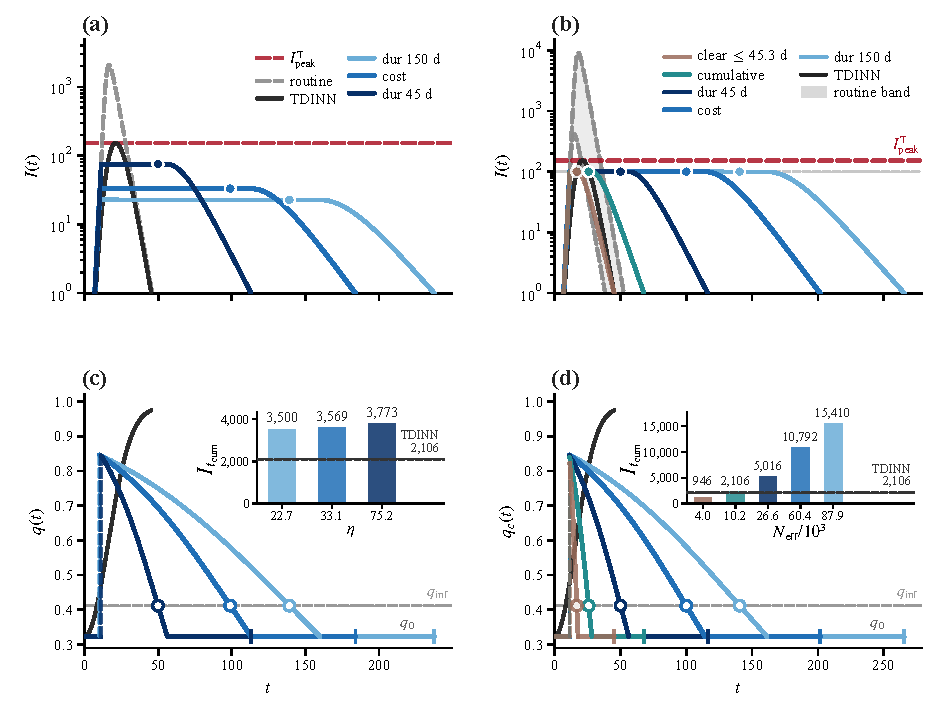
\includegraphics[width=\textwidth]{figures/layout_v5/population_threshold_levers.pdf}
\caption{阈值与有效人口对轨迹的不同影响。左列固定 $N_{\rm eff}=20000$，$\eta=22.7,33.1,75.2$ 分别对应 $150$ d 时长、成本和 $45$ d 时长条件；右列固定 $\eta=100$，清零、累计新增感染、$45$ d 时长、成本和 $150$ d 时长条件分别对应 $N_{\rm eff}\approx3973,10151,26584,60424,87944$。前两个人口规模低于 $N_{\rm floor}$，仅用于展示边界外的轨迹。(a)、(b) 为社区感染者人数；(c)、(d) 为隔离比例；横轴 $t$ 的单位为天。黑实线为固定 TDINN 参照，红虚线为其感染峰值；左列灰虚线为同人口常规控制，右列灰带为常规轨迹范围。空心圆标记隔离比例拐点，水平段上的实心点是该时刻在感染曲线上的投影，并非感染曲线自身的拐点；短竖线表示清零时间。内嵌柱图给出清零时的总累计新增感染，虚线为 TDINN 参照 $2105.63$。}
\label{fig:dom:levers}
\end{figure}

例如，$N=5\times10^4$、$\eta=100$ 的已计算情景满足峰值、成本及 $T_{\max}=150$ 天的要求，$J=40.77$、$\Delta t=85.07$ 天。累计新增感染约为 $9.03\times10^3$ 人、清零时间约为 $176$ 天，均超过 TDINN 参照值；该点说明峰值与成本条件不足以保证其余两项指标达标。

\subsection{不同有效人口下的轨迹分解与临界案例}
\label{app:panel_eta_N}
固定 $\eta=100$ 时的分人口轨迹见图\ref{fig:panel_N_decomp}。

\begin{figure}[htbp]
\centering
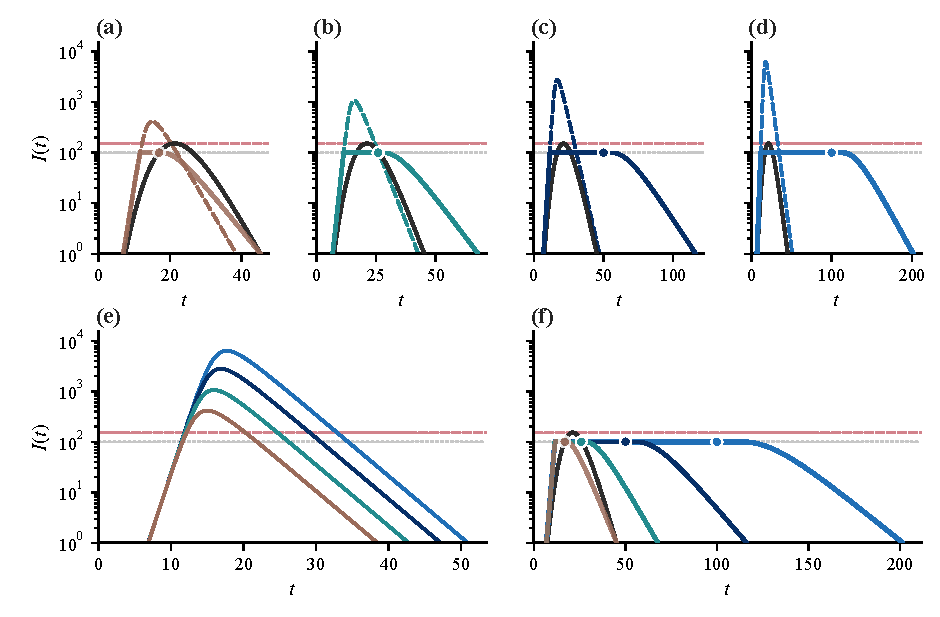
\includegraphics[width=\textwidth]{figures/layout_v5/fig_panel_B_trajectory_decomposition.pdf}
\caption{固定 $\eta=100$ 时不同有效人口下的感染轨迹。(a)--(d) 分别对应 $N_{\rm eff}=3973,10151,26584,60424$，各包含阈值控制、常规控制和固定 TDINN 参照；(e) 比较四个人口规模下的常规控制；(f) 比较阈值控制与 TDINN。横轴 $t$ 的单位为天。}
\label{fig:panel_N_decomp}
\end{figure}
三类临界有效人口下的阈值比较见图\ref{fig:dom:critical-cases}。
\clearpage
\begin{figure}[H]
\centering
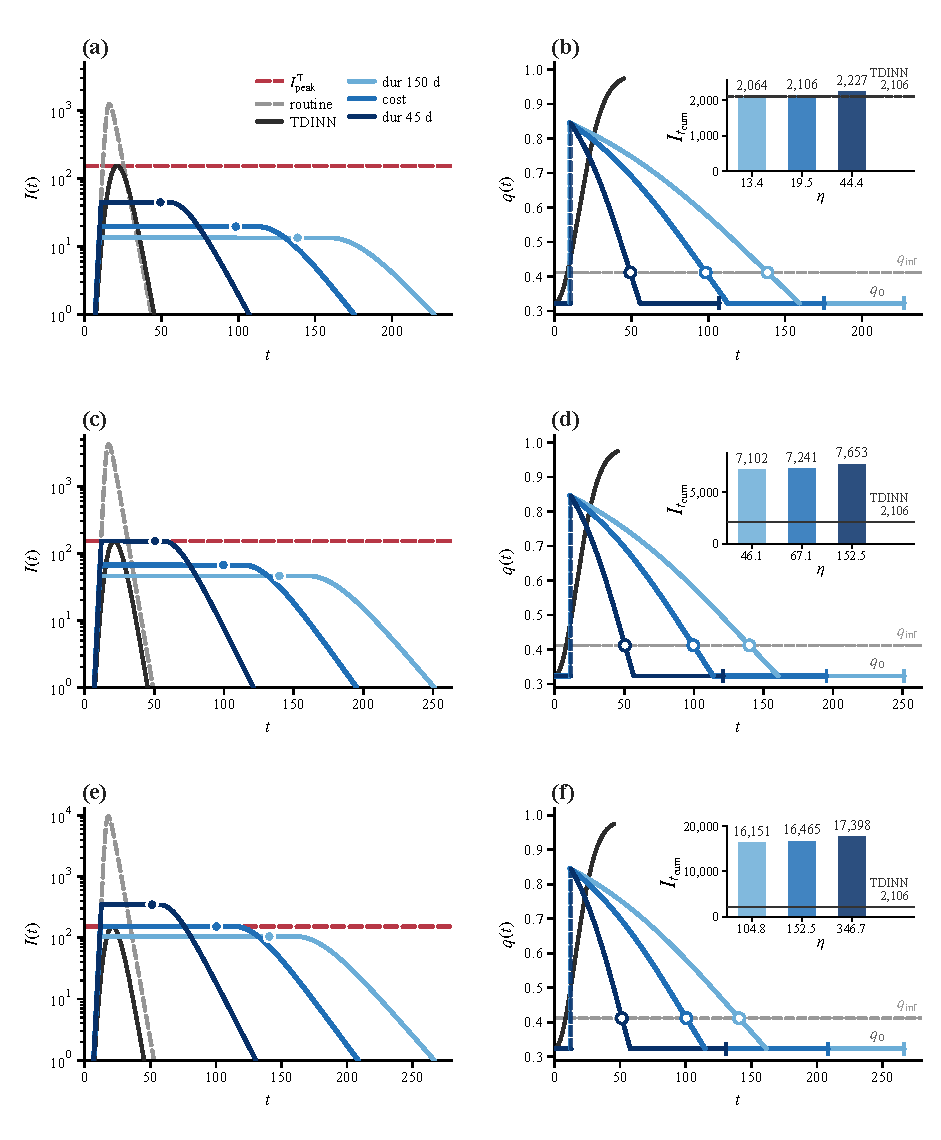
\includegraphics[width=\textwidth]{figures/layout_v5/critical_population_cases.pdf}
\caption{三类临界有效人口下的阈值比较。三行依次为 $N_{\rm eff}=11813,40553,92174$；左列为社区感染者人数（对数纵轴），右列为隔离比例，横轴 $t$ 的单位为天。(a) 中的图例适用于三行：蓝色轨迹对应 $150$ d 时长、成本和 $45$ d 时长条件，黑实线为固定 TDINN 参照，灰虚线为同人口常规控制，红虚线为 TDINN 感染峰值。空心圆标记隔离比例拐点，水平段上的实心点为该时刻在感染曲线上的投影而非感染曲线的拐点，短竖线为清零时间。内嵌柱图给出清零时的总累计新增感染，虚线为 TDINN 参照 $2105.63$。}
\label{fig:dom:critical-cases}
\end{figure}

本小节采用三个阈值比例：
\[
\theta_{\rm dur150}=1.137\times10^{-3},\qquad
\theta_{\rm cost}=1.655\times10^{-3},\qquad
\theta_{\rm dur45}=3.762\times10^{-3}.
\]
初值仍取固定绝对值 $I_0$，不同 $N_{\rm eff}$ 下不重新拟合。三个人口规模分别对应累计新增感染、45天控制时长和成本条件的临界值，结果见图\ref{fig:dom:critical-cases}。各参数组中，拐点相对位置约为 $\lambda=0.861$，绝对时刻随启动时间改变。

当 $N_{\rm eff}=11813$ 时，三个阈值为 $13.432,19.550,44.435$，清零时间分别约为 $227.6,175.5,107.1$ d；成本条件下累计新增感染约为 TDINN 参照 $2105.63$，另外两个阈值的结果分别低于和高于该参照。当 $N_{\rm eff}=40553$ 时，三个阈值为 $46.113,67.115,152.546$，最后一个约等于 TDINN 峰值。当 $N_{\rm eff}=92174$ 时，三个阈值为 $104.810,152.546,346.725$，分别低于、约等于和高于 TDINN 峰值。



\FloatBarrier
\subsection{传播概率的影响与比较边界的数值结果}
\label{app:dom:numerics}

传播概率扫描和两项指标的等值线计算点给出候选边界的数值范围。

固定乘积 $\beta c_0=1.9305$，在 $\beta\in[0.10,0.30]$ 内，候选人口范围的两个端点随 $\beta$ 改变，但端点比值变化较小：
$N^\ast_\infty/N_{\rm floor}\in[8.675,\,8.694]$，极差 $0.22\%$（$\beta=0.10/0.1498/0.20/0.30$ 处
$N^\ast_\infty=13.55/9.22/7.03/4.86\times10^4$、$N_{\rm floor}=1.56/1.06/0.81/0.56\times10^4$）。
$\beta N^\ast_\infty$ 与 $\beta N_{\rm floor}$ 各自随 $\beta$ 漂移约 $7.6\%$ 与 $7.8\%$，
二者的变化幅度接近，但都不严格正比于 $1/\beta$。

在 $\eta\in[10,152.55]$ 内，累计新增感染等值曲线 $\Itcum(\eta,N)=\Itcum^{\rm T}$ 从 $(9511,152.55)$ 延伸至 $(12230,10)$，$\eta=100$ 时 $N_{\rm cum}\approx1.015\times10^4$。它与实际成本条件的数值交点约为 $(11813,19.55)$，给出 $N_{\rm cum,\infty}^\ast\approx1.18\times10^4$，约为 $N^\ast_\infty$ 的 $0.13$。现有 $16$ 个计算点及其插值仅显示一次交点，尚不能据此确定一般参数下交点的唯一性。

$t_{\rm end}=t_{\rm end}^{\rm T}$ 在同一阈值范围内从 $(866.4,\,10)$ 延伸到 $(5184.4,\,152.55)$，
$\eta=100$ 处 $N_{\rm clr}\approx3.97\times10^{3}$，已有计算点及插值中的最大人口值为 $N=5184$。

本小节的累计新增感染均计算至各策略的清零时间，包含退出后的感染过程。

\FloatBarrier

\subsection{仅隔离控制与给定参照指标的比较条件}
\label{app:reference-comparison}
本小节给出正文第\ref{sec:s1}节仅隔离控制的人口尺度比较条件。固定归一化初值 $s_0,i_0$ 和其余参数，记 $i_{\max}^{no}=I_{\max}^{no}/N$。由命题\ref{prop:threshold-tradeoff}和\ref{prop:scaling}，$\Delta t(\theta)$ 和 $J(\theta)$ 在 $(i_0,i_{\max}^{no})$ 上严格递减，右端极限为零，左端极限 $\Delta t(i_0+)$、$J(i_0+)$ 均有限且为正。下述人口上界商式仅用于这一初值约定；固定绝对初值的应用上界按第\ref{sec:dom:xian}节的实际指标定义。

给定正的成本参照 $J^{\rm T}$ 和允许时长 $T_{\max}$，沿用正文的阈值记号，作如下端点扩展：
\begin{equation}
\theta_{\rm cost}=\begin{cases}
J(\theta)=J^{\rm T}\text{ 的唯一根},&0<J^{\rm T}<J(i_0+),\\
i_0,&J^{\rm T}\ge J(i_0+),
\end{cases}
\label{eq:reference-cost-threshold}
\end{equation}
\begin{equation}
\theta_{\rm dur}(T_{\max})=\begin{cases}
\Delta t(\theta)=T_{\max}\text{ 的唯一根},&0<T_{\max}<\Delta t(i_0+),\\
i_0,&T_{\max}\ge\Delta t(i_0+)\text{ 或不限制时长}.
\end{cases}
\label{eq:reference-duration-threshold}
\end{equation}
端点值 $i_0$ 表示相应比较条件对全部内部触发阈值成立，不表示将 $\theta=i_0$ 纳入内部触发。令 $\theta_{\rm bind}=\max\{\theta_{\rm cost},\theta_{\rm dur}(T_{\max})\}$。给定峰值参照 $I^{\rm T}_{\rm peak}>0$，则同时满足峰值、成本与时长条件的阈值比例集合恰为
\begin{equation}
(i_0,i_{\max}^{no})\cap
\left[\theta_{\rm bind},\frac{I^{\rm T}_{\rm peak}}{N}\right].
\label{eq:reference-feasible-set}
\end{equation}
这一结论由 $J,\Delta t$ 的单调性和 $\eta=\theta N$ 直接得到。上述定义保证 $\theta_{\rm bind}<i_{\max}^{no}$。当 $\theta_{\rm bind}>i_0$ 时，集合非空等价于 $N\le I^{\rm T}_{\rm peak}/\theta_{\rm bind}$；当 $\theta_{\rm bind}=i_0$ 时，条件改为严格不等式 $N<I^{\rm T}_{\rm peak}/i_0$。固定正 $i_0$ 时，$T_{\max}\to\infty$ 对应 $\theta_{\rm dur}\to i_0$，不是零。

\begin{proposition}
\label{prop:reference-population}
固定 $s_0,i_0,\theta$ 和模型参数，且 $i_0<\theta<i_{\max}^{no}$。在 $N\theta>1$ 的范围内，仅隔离控制的清零时间和计算至该终点的累计新增感染均随 $N$ 严格增加。
\end{proposition}
\begin{proof}
归一化轨迹及启动、控制时长与 $N$ 无关。退出后 $i(t)$ 从 $\theta$ 严格下降至零，终点为 $i=1/N$。增大 $N$ 使终点更低，故清零时间严格增加。

记 $s_{\rm end}=S_{\rm end}/N$。归一化的退出后首次积分为
\[
\frac1N=\theta+\frac{\beta_2^0}{\beta_1^0}(s_c-s_{\rm end})
+\frac{\rho_1}{N}\ln\frac{s_{\rm end}}{s_c},
\]
其中 $\rho_1/N$ 与 $\beta_2^0/\beta_1^0$ 均不随 $N$ 改变。于是
\[
\frac{\partial s_{\rm end}}{\partial N}
=-\frac1{N^2(\rho_1/N)(1/s_{\rm end}-1/s_c)}<0.
\]
将式\eqref{eq:s1:cumulative}除以 $N$ 后，只有 $s_{\rm end}$ 含 $N$，因而
\[
\frac{\partial\Itcum}{\partial N}
=\frac{\Itcum}{N}
-\frac{N\beta}{\beta+q_0(1-\beta)}\frac{\partial s_{\rm end}}{\partial N}>0.\qedhere
\]
\end{proof}
该命题针对固定 $\theta$、固定归一化初值的人口变化，不能直接用于固定绝对 $\eta$ 或固定绝对 $I_0$ 的比较。累计新增感染与清零等值线的存在和交点唯一性，应按实际采用的初值及参数变化方向分别说明。

若还要求候选人口容纳给定参照轨迹，则由式\eqref{eq:count-identities}有必要条件 $N\ge I^{\rm T}_{\rm cum}+I^{\rm T}_{q_{\rm cum}}/\beta$。这一下界不是有效人口的估计，也不保证候选人口能重现参照数据。上述条件描述给定指标下的条件性比较，不构成不同传播人口之间的因果政策比较。


\FloatBarrier
